\section{Analysis and Results}\label{sec:results}
% \subsection{Expected behaviour}
This section shows the analysis of the system presented in the previous section and its behaviour.

% \subsection{Static}
\subsection{Frequency}
In order to determine whether the proposed method yields an output with the correct frequency content in the static case, a spectrum is taken of the system's output. The system with $N=15.5$ (so $\alpha = 0.5$ in \eqref{eq:bMat}) at a sample rate of $f_\text{s} = 44100$ Hz is compared to the same system with $f_\text{s} = 88200$ Hz resulting in $N=31$ ($\alpha = 0$) for the same $f_0$ according to Eq. \eqref{eq:fundamentalFreq}. See Figure \ref{fig:spectra}.

\begin{figure}[ht]
    \centering
%% \reprintcolumnwidth is the same in preprint and reprint for
%% ease of use for authors:
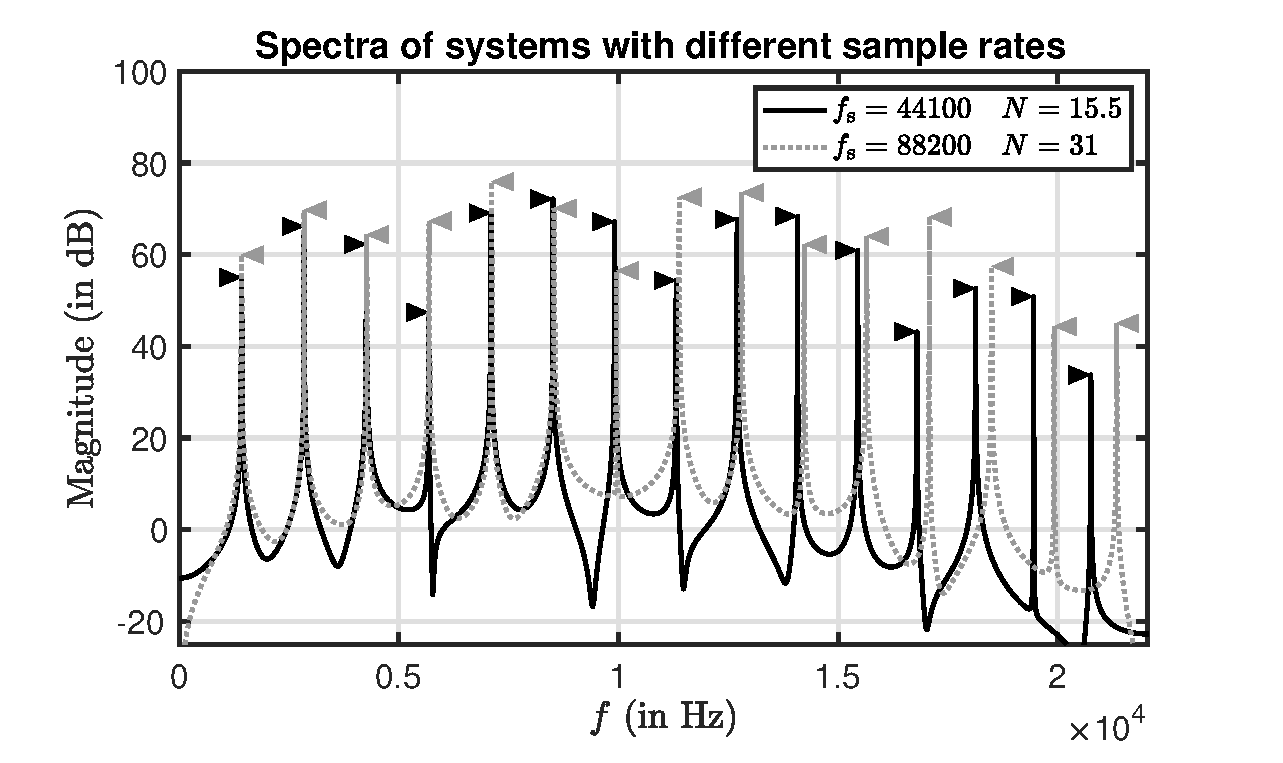
\includegraphics[width=0.8\columnwidth]{Figures/spectraDoubleSampleRateQuadratic.eps}
\caption{\label{fig:spectra}{A system with $N = 15.5$ at $f_\text{s} = 44100$} compared to a system with $N = 31$ at $f_\text{s} = 88200$. Both are supposed to have the same fundamental frequency $f_0$ according to Eq. \eqref{eq:fundamentalFreq}.}
\end{figure} 

As expected, the output of the system at integer $N = 31$ contains partials at perfect integer multiples of $f_0$ (Eq. \eqref{eq:fundamentalFreq}). When this is compared to the output of the system with $N = 15.5$, one can observe that the lower partials are nearly perfectly overlapping, whereas higher partials exhibit slight downwards deviations, exponentially increasing with frequency.

% \subsection{Dynamic}
For a more detailed look at the behaviour of the system when $c$ is changed dynamically, a modal analysis can be performed on system \eqref{eq:totalSystem}. For slow variations of $c$, the modal frequency of the $p$'th mode can be retrieved as
\begin{equation}\label{eq:modalAnalysis}
    f_p \approx \frac{1}{2\pi k}\cos^{-1}\left(\frac{1}{2}\text{eig}_p(\mathbf{B})\right).
\end{equation}
In the following, $f_\text{s} = 44100$.
As a test case, the wave speed is dynamically varied from $c = 2940$ ($N = 15$) to $c = 2205$ ($N = 20$), changing $\mathbf{B}$ and thus the modal frequencies over time. The displacement correction presented in Eq. \eqref{eq:dispCorr} is not included in this analysis ($\epsilon \gg 1$), but will be elaborated on in Section \ref{sec:dispCorrRes}. The results of the analysis are shown in Figure \ref{fig:modalAnalysis}. Figure \ref{fig:spectrogram} shows the resulting spectrogram of the system excited at $n=0$ with a narrow raised cosine and the output retrieved at $u_1$.

\begin{figure}[ht]
    \centering
%% \reprintcolumnwidth is the same in preprint and reprint for
%% ease of use for authors:
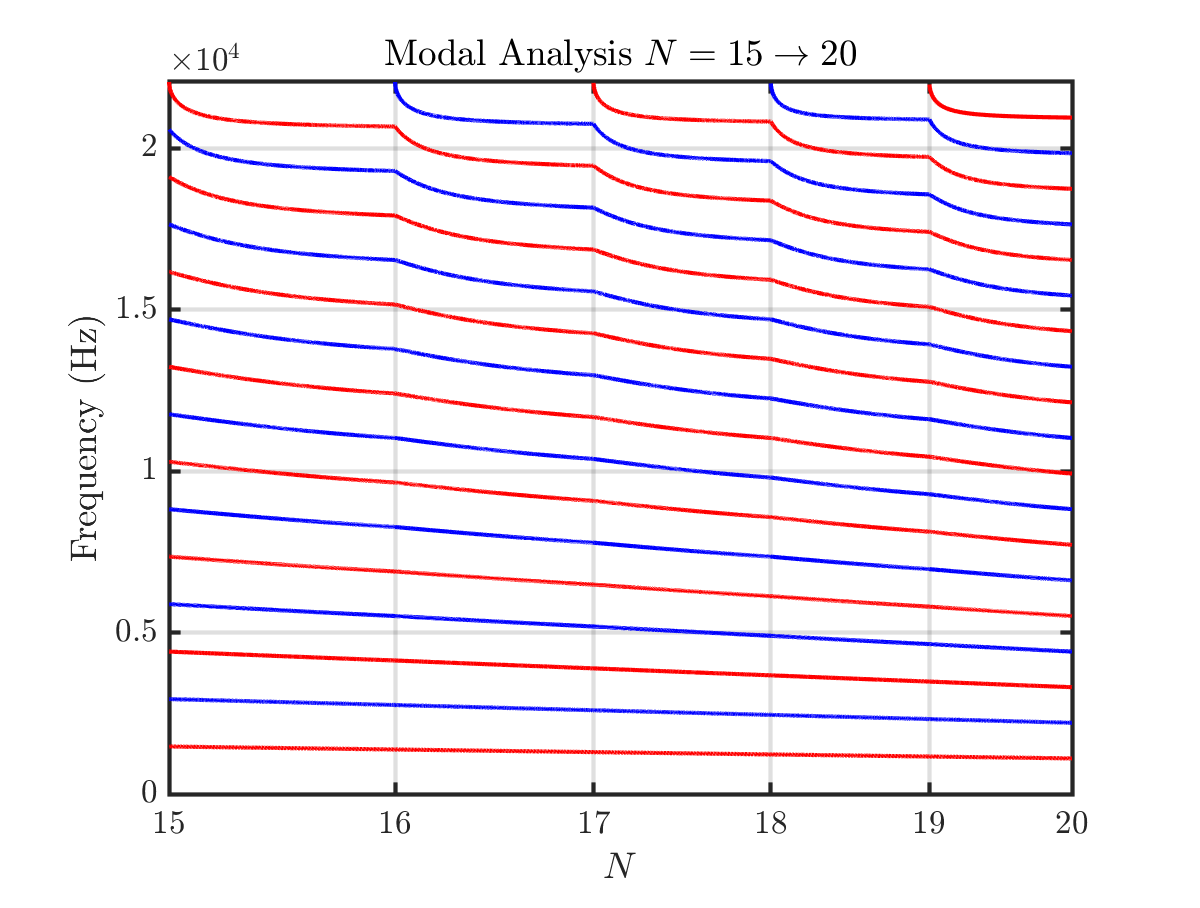
\includegraphics[width=\figwidth\columnwidth]{Figures/modalAnalysisQuadratic.eps}
\caption{\label{fig:modalAnalysis}{Modal analysis of system \eqref{eq:totalSystem} using \eqref{eq:modalAnalysis}. The wave speed is reduced from $c = 2940$ ($N = 15$) to $c = 2205$ ($N = 20$).}}
\end{figure} 
\begin{figure}[ht]
    \centering
%% \reprintcolumnwidth is the same in preprint and reprint for
%% ease of use for authors:
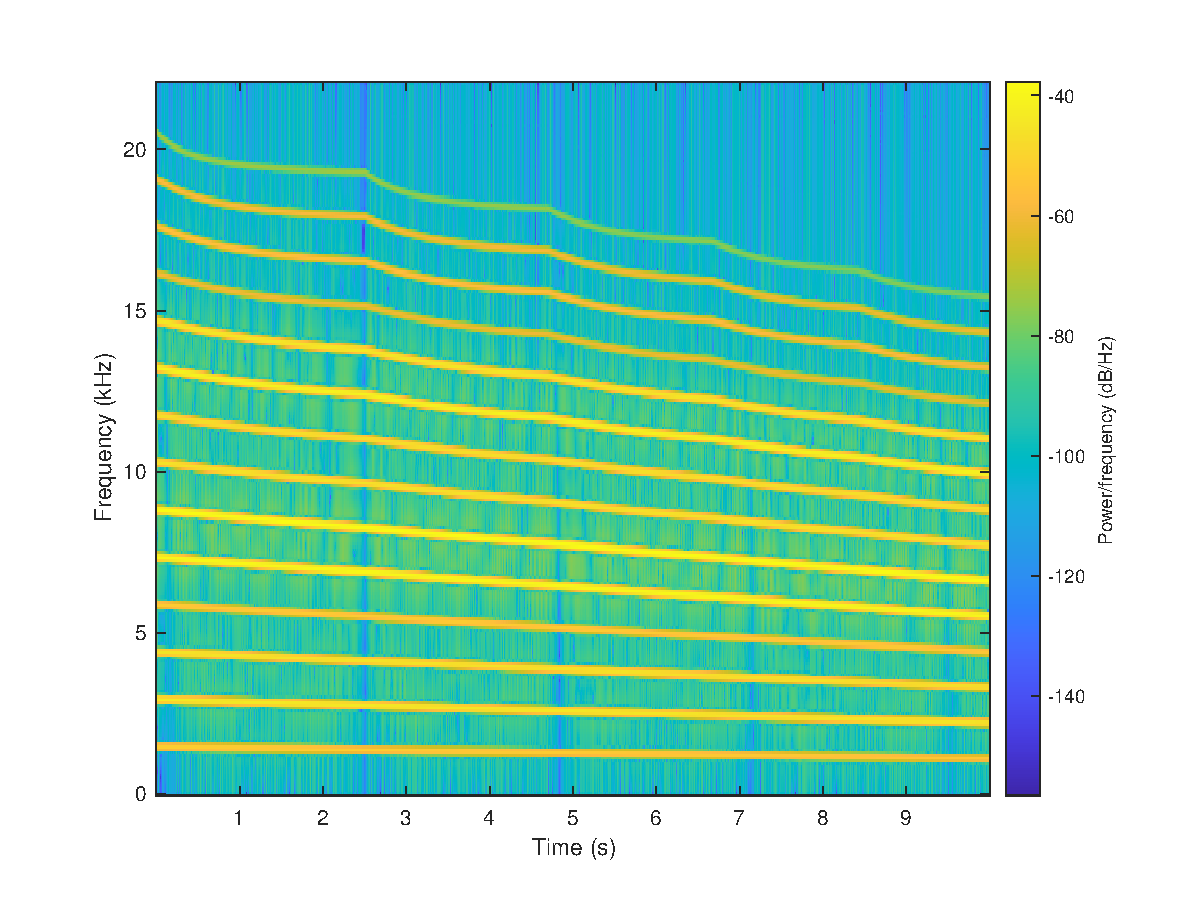
\includegraphics[width=\figwidth\columnwidth]{Figures/specQuadratic.eps}
\caption{\label{fig:spectrogram}{System output. The sound output follows the same pattern as predicted by the analysis shown in Figure \ref{fig:modalAnalysis}.}}
\end{figure} 

In the following \SWcomment[came up with this measure myself.. it made sense to me for measuring harmonic deviation / inharmonicity. Please let me know if you know a better measure or something I can reference]
\begin{equation}
    \varepsilon_p = \frac{f_p - pf_0}{f_0}\quad \text{[\%]}
\end{equation}
is used to calculate the harmonic deviation of mode $p$ from an integer multiple of the fundamental. Furthermore, the lowest mode generated by the analysis is referred to as $f_1$ and should ideally be equal to $f_0$ calculated using Eq. \eqref{eq:fundamentalFreqCont}.

The first thing one can observe from Figure \ref{fig:modalAnalysis} is that the frequencies of the modes decrease as $c$ decreases. The lower the mode, the more linear this decrease happens. Between $N = 15$ and $N = 16$, $f_1$ maximally deviates by $-0.12$ Hz or $\varepsilon_1 = -0.008\%$. In this same interval $f_{15}$ maximally deviates by $-827.15$ Hz or $\varepsilon_{15} = -57\%$. This deviation for mode number $p$ gets progressively less as $N$ increases. The maximum deviation for the highest mode number $f_{\lfloor N\rfloor}$, however, gets larger with a larger $N$, with $\text{max}(\varepsilon_{\lfloor N \rfloor})$ approaching $-100\%$ for extremely large values of $N$ ($>1000$). These deviations only happen between integer values of $N$ where at integer $N$ all modes are perfect integer multiples of $f_0$ and $\varepsilon_p = 0 \%$ for all $p$.

Experiments with higher even-ordered Lagrange interpolators shows that $\varepsilon_p$ becomes smaller, but not by a substantial amount. The quadratic interpolator has thus been chosen for being simpler and more flexible while not being substantially worse than higher order interpolators.

Another observation from Figure \ref{fig:modalAnalysis} is that there are always $\lfloor N \rfloor$ modes present, corresponding to the number of moving points of the system. As can be seen from the spectrum in Figure \ref{fig:spectrogram} the highest mode is not excited. When an implementation of the system using this method, with wave speed $c = 2940$ m/s (static) is compared to a normal implementation of the 1D wave equation (shown in Section \ref{sec:FDTD}) with the same wavespeed, identical outputs are observed, even though the latter has $N-1$ moving points. This proves that at integer $N$ the method reduces to the normal case. If the system is excited when $N$ is not an integer, the highest mode will also be excited.

Using the quadratic interpolation from \eqref{eq:connectionInterpol}, or any other even-ordered Lagrange interpolator for that matter, the modal behaviour of the system does not change based on location. Experiments done with odd-ordered Lagrange interpolators showed that better behaviour is observed when points are added / removed closer to the boundaries. 

\subsection{Displacement Correction}\label{sec:dispCorrRes}
(FIR) Comb filtering effect where resonances appear depending on the location of correction. Middle has least

\subsection{Limit on Speed of Change}
The method presented in this paper can only add or remove a maximum one point per sample using Eqs. \eqref{eq:addingPoint} and \eqref{eq:removingPoint}. The speed of decreasing $f_0$ according to \eqref{eq:fundamentalFreq} is thus limited by the following condition
\begin{equation}\label{eq:pointCondition}
    |N^n - N^{n-1}| \leq 1. 
\end{equation}
Though this is the maximal limitation on speed, a much lower limitation needs to be placed to keep the system well-behaved.  

The usual stability and energy analyses performed on FDSs are not valid anymore in the time-varying case. Frozen coefficient analysis as in [REF] can be applied here for slowly varying coefficients, but is left for future work. 
% Notes:
% In the case that $\alpha = 0$ in Eq. \eqref{eq:totalSystem} (and thus $x_{u_M} = x_{w_0}$), one could go up to adding two points at a time by adding $u_{M+1}^n$ according to Eq. \eqref{eq:addingPoint} and adding an extra point $u_{M+2}^n$ using \eqref{eq:calcVirtualGridPoints} (in this case $u_{M+2}^n = w_0^n$). This would, however, not work if $\alpha \neq 0$, as a point added to $\mathbf{u}^n$ with $x_\text{i} < w_0$ needs interpolator \eqref{eq:customIp} and $\alpha'$ would be greater than $1$. As Eq. \eqref{eq:customIp} only works if $0\leq \alpha' \leq 1$, it is best to abide condition \eqref{eq:pointCondition} to be safe. 

% No speed limit if
% \begin{equation}
%     \text{floor}(N^n) = \text{floor}(N^{n-1})\Rightarrow M^n = M^{n-1},
% \end{equation}
% i.e., if no points are added or removed from the system. 